On étudie la croissance d'une population de champignons.

\subsubsection*{Partie A}
Au début de l'expérience, on dispose de 100 champignons. Toutes les dix minutes, on mesure l'évolution de leur nombre. On obtient les résultats suivants :

\begin{minipage}[t]{0.5\textwidth}
\centering

\begin{tabular}{|c|c|}
\hline
\makecell{Temps écoulé \\ (en minutes)} & \makecell{Nombre de \\ champignons} \\
\hline
0 & 100 \\
10 & 125 \\
20 & 150 \\
30 & 175 \\
\hline
\end{tabular}

\end{minipage}
\hfill
\begin{minipage}[t]{0.45\textwidth}
\vspace{-1.5cm}
\centering

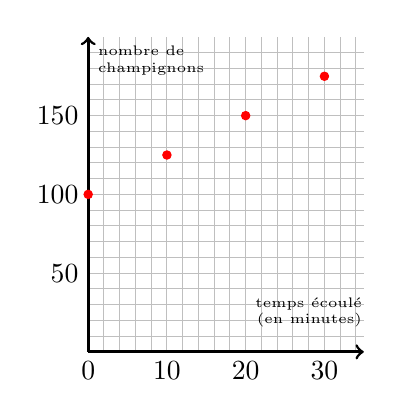
\begin{tikzpicture}[scale=0.1]
\foreach \x in {0,10,...,35} {
\draw[gray] (\x,0) -- (\x,40);
}
\foreach \y in {0,50,...,190} {
\draw[gray] (0,\y/5) -- (35,\y/5);
}
\foreach \x in {0,2,...,35} {
\draw[lightgray] (\x,0) -- (\x,40);
}
\foreach \y in {0,10,...,190} {
\draw[lightgray] (0,\y/5) -- (35,\y/5);
}
\draw[->, line width=1pt] (0,0) -- (35,0) node[]{};
\draw[->, line width=1pt] (0,0) -- (0,40) node[]{};
\node[align=right, font=\tiny] at (28,5) {temps écoulé\\ (en minutes)};
\node[align=left, font=\tiny] at (8,37) {nombre de\\ champignons};
\foreach \x in {0,10,20,30} {
\draw (\x,0) node[below]{$\x$};
}
\foreach \y in {50,100,150} {
\draw (0,\y/5) node[left]{$\y$};
}
\foreach \x/\y in {0/100, 10/125, 20/150, 30/175} {
\filldraw[red] (\x,\y/5) circle (15pt);
}
\end{tikzpicture}

\end{minipage}

Soit $n$ un entier naturel. On note $u_n$ le nombre de champignons après $n$ périodes de \textbf{dix} minutes. Ainsi $u_0 = 100$, $u_1 = 125$, $u_2 = 150$...

\begin{enumerate}
\item Justifier que les termes $u_0$, $u_1$, $u_2$, $u_3$ sont en progression arithmétique.

\item En supposant que la population de champignons continue d'évoluer selon le même rythme, montrer qu'elle aura quadruplé deux heures après le début de l'expérience.
\end{enumerate}

\begin{minipage}[t]{0.6\textwidth}
\subsubsection*{Partie B}
En réalité, on constate que la population de champignons a quadruplé 80 minutes après le début de l'expérience. De nouvelles mesures donnent les résultats suivants.
\end{minipage}
\hfill
\begin{minipage}[t]{0.35\textwidth}
\vspace{0pt}
\begin{center}
\begin{tabular}{|c|c|}
\hline
\makecell{Temps écoulé \\ (en minutes)} & \makecell{Nombre de \\ champignons} \\
\hline
0 & 100 \\
40 & 200 \\
80 & 400 \\
120 & 800 \\
\hline
\end{tabular}
\end{center}
\end{minipage}

Soit $n$ un entier naturel. On note $v_n$ le nombre de champignons, après $n$ périodes de \textbf{quarante} minutes. Ainsi $v_0 = 100$, $v_1 = 200$, $v_2 = 400$...

\begin{enumerate}
\item Montrer que les termes $v_0$, $v_1$, $v_2$, $v_3$ sont en progression géométrique.

\item On suppose que la suite $(v_n)$ est une suite géométrique de raison 2.

Indiquer sans justifier lequel des 4 graphiques ci-dessous est susceptible de représenter la suite $(v_n)$.
\end{enumerate}

\begin{minipage}[t]{0.24\textwidth}
\begin{center}
Graphique 1 \\
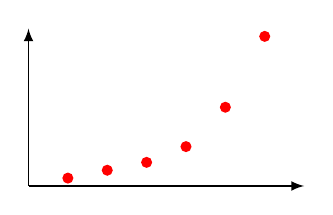
\begin{tikzpicture}
\draw[semithick,->,>=latex] (0,0) -- (3.5,0) ;
\draw[semithick,->,>=latex] (0,0) -- (0,2) ;
\foreach \coord in {(0.5,0.1),(1,0.2),(1.5,0.3),(2,0.5),(2.5,1),(3,1.9)} {
        \fill[red] \coord circle (2pt);
    }
\end{tikzpicture}
\end{center}
\end{minipage}
\hfill
\begin{minipage}[t]{0.24\textwidth}
\begin{center}
Graphique 2 \\
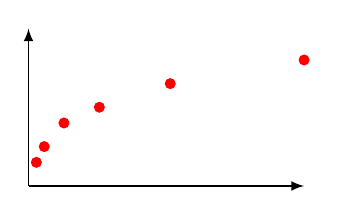
\begin{tikzpicture}
\draw[semithick,->,>=latex] (0,0) -- (3.5,0) ;
\draw[semithick,->,>=latex] (0,0) -- (0,2) ;
\foreach \coord in {(0.1,0.3),(0.2,0.5),(0.45,0.8),(0.9,1),(1.8,1.3),(3.5,1.6)} {
        \fill[red] \coord circle (2pt);
    }
\end{tikzpicture}
\end{center}
\end{minipage}
\hfill
\begin{minipage}[t]{0.24\textwidth}
\begin{center}
Graphique 3 \\
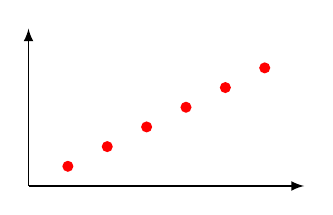
\begin{tikzpicture}
\draw[semithick,->,>=latex] (0,0) -- (3.5,0) ;
\draw[semithick,->,>=latex] (0,0) -- (0,2) ;
\foreach \coord in {(0.5,0.25),(1,0.5),(1.5,0.75),(2,1),(2.5,1.25),(3,1.5)} {
        \fill[red] \coord circle (2pt);
    }
\end{tikzpicture}
\end{center}
\end{minipage}
\hfill
\begin{minipage}[t]{0.24\textwidth}
\begin{center}
Graphique 4 \\
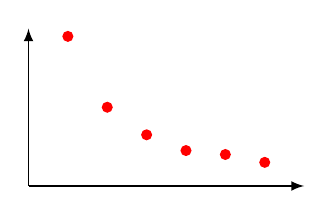
\begin{tikzpicture}
\draw[semithick,->,>=latex] (0,0) -- (3.5,0) ;
\draw[semithick,->,>=latex] (0,0) -- (0,2) ;
\foreach \coord in {(0.5,1.9),(1,1),(1.5,0.65),(2,0.45),(2.5,0.4),(3,0.3)} {
        \fill[red] \coord circle (2pt);
    }
\end{tikzpicture}
\end{center}
\end{minipage}

\begin{center}
\begin{minipage}{0.75\textwidth}
\begin{enumerate}[start=3]
\item Quel sera le nombre de champignons quatre heures après le début de l'expérience ?

\item Cinq heures après le début de l'expérience, on dénombre environ 18 000 champignons. Est-ce cohérent avec le modèle choisi ?
\end{enumerate}
\end{minipage}
\hfill
\fbox{
\begin{minipage}{0.2\linewidth}
\centering
Aide au calcul :

$2^6 = 64$

$2^7 = 128$

$2^8 = 256$

$2^9 = 512$

$2^{10} = 1024$
\end{minipage}
}
\end{center}
